%% Basic Academic Journal Article Template
%% Author
%% John Hammersley
%% License
%% Creative Commons CC BY 4.0
%% Abstract
%% This is a basic journal article template which includes metadata fields for multiple authors, affiliations and keywords.

%% It is also set up to use the lineno package for line numbers; these can be turned on by adding the 'lineno' option to the documentclass command.

%% Tags
%% Find More Templates
%% Basic Academic Journal Article Template
%% © 2020 OverleafPrivacy and TermsSecurityContact UsAboutBlog
%% Overleaf on TwitterOverleaf on FacebookOverleaf on LinkedIn
\documentclass[fleqn,12pt]{olplainarticle}

% Use option lineno for line numbers 

\usepackage[utf8]{inputenc}
\usepackage{graphicx}
\usepackage{hyperref}
\usepackage{microtype}
\usepackage{lineno}
\linenumbers

\title{Genotypic variation in a foundation tree results in heritable
  ecological network structure}

\author[1,2]{Matthew K. Lau}
\author[1,3,4]{Louis J. Lamit}
\author[1,5]{Rikke Reese Næsborg}
\author[6]{Stuart R. Borrett}
\author[7]{Matthew A. Bowker}
\author[1,8]{Thomas G. Whitham}

\affil[1]{Department of Biological Sciences, Northern Arizona
  University, Flagstaff, AZ 86011, USA}
\affil[2]{Harvard Forest, Harvard University, 324 N Main St,
  Petersham, MA 01366, USA}
\affil[3]{Department of Biology, State University of New York College
  of Environmental Sciences, Syracuse University, 107 College
  Place Syracuse, NY 13244, USA}
\affil[4]{Department of Environmental Forest Biology and Forestry,
  Syracuse, NY 13210, USA}
\affil[5]{Santa Barbara Botanic Garden, 1212 Mission Canyon Road,
  Santa Barbara, CA 93105}
\affil[6]{Department of Biology and Marine Biology, University of
  North Carolina Wilmington, 601 South College Road, Wilmington, NC
  28403, USA}
\affil[7]{Duke Network Analysis Center, Duke University, Durham, NC
  27708, USA}
\affil[8]{School of Forestry, 200 E. Pine Knoll Dr., Northern Arizona
  University, Flagstaff, AZ 86011, USA}
\affil[9]{Center for Adaptable Western Landscapes, Northern Arizona
  University, Flagstaff, AZ 86011, USA}

\keywords{networks $|$ heritability $|$ community $|$ genetics $|$
  lichen $|$ cottonwood $|$ \textit{Populus} $|$ common garden}

%% \significancestatement{Evolution occurs in the context of ecosystems
%%   comprised of complex ecological networks. Research at the interface
%%   of ecology and evolution has primarily focused on pairwise
%%   interactions among species and have rarely included a genetic
%%   component to network structure. Here, we used a 20+ year common
%%   garden experiment to reveal the effect that genotypic variation can
%%   have on networks of lichens that colonize the bark of a foundation
%%   tree species. We found that lichen interaction network structure is
%%   genetically based and primarily driven by bark roughness. These
%%   findings demonstrate the importance of genetic variation and
%%   evolutionary dynamics in shaping ecological networks as evolved
%%   traits. In particular, this study points to the importance of
%%   assessing the effect of foundation species genetics on the structure
%%   of species interactions that can generate heritable network
%%   variation that selection can act upon.}


\begin{abstract}

%% Currently: 250 words (Thu 05 Nov 2020 10:55:40 AM EST)
  
Elucidating the genetic basis to ecological network structure is
fundamental to understanding evolution in complex ecosystems. Although
previous work has demonstrated that genetic variation can influence
food webs and trophic chains, we are unaware of a study that
quantified the contribution of phenotypic variation to heritable
variation in network structure. To examine this, in a 20+ year old
common garden we observed epiphytic lichens associated with narrowleaf
cottonwood (\textit{Populus angustifolia}), a riparian ecosystem
foundation species. We constructed and conducted genetic analyses of
signed, weighted, directed lichen interaction networks on individual
trees. We found three primary results. First, genotype identity
significantly predicted lichen network similarity; i.e., replicates of
the same genotype supported more similar lichen networks than
different genotypes. Second, broad sense heritability estimates showed
that plant genotype explained network similarity ($H^2$ = 0.41),
degree ($H^2$ = 0.32) and centralization ($H^2$ = 0.33). Third, of
several tree phenotypic traits examined, bark roughness was both
heritable ($H^2$ = 0.32) and significantly predicted by lichen network
similarity ($R^2$ = 0.26). These results support a mechanistic,
genetic pathway from variation in a heritable tree trait to ecological
network structure and demonstrate that evolution can act at the
community level to influence not only abundances of organisms but also
interactions at the scale of entire networks. Given that network
structure can influence system-wide stability and resilience, which
creates potential for selection to act at the community level, our
findings have important implications for how evolution acts in
ecosystems.

\end{abstract}

\begin{document}

\flushbottom
\maketitle
\date
\thispagestyle{empty}

\section*{Introduction}

Evolution occurs in the context of complex ecological
networks. Community genetics studies have shown that genetic variation
in foundation species, which have large effects on ecosystems by
modulating and stabilizing local conditions \citep{Ellison2005}, plays
a significant role in defining distinct communities of interacting
organisms: such as endophytes, pathogens, lichens, arthropods, and
soil microbes \citep{Busby2015, Barbour2009c, Lamit2015c}. Multiple
studies have now demonstrated that genetic variation influences
numerous functional traits (e.g., phytochemical, phenological,
morphological) that in combination result in a multivariate functional
trait phenotype \citep{holeski2012} in which individual plant
genotypes support different communities and ecosystem processes
\citep{Bailey2009a, Whitham2012}. Recently, the importance of genetic
variation in structuring ecological systems was reviewed, and not only
were many instances of strong genetic effects found in many ecosystems
but the effect of intraspecific variation was at times greater than
inter-specific variation \citep{DesRoches2018TheVariation}. There is
now evidence to support that selection, acting on this heritable
variation, tends to occur among groups of species
\citep{Wade2007TheCommunities} and that genetic variation and
phylogenetic relatedness contribute to variation in community assembly
\citep{Crutsinger2016} and species interactions \citep{Whitham2006a,
  Bailey2009a, Moya-Larano2011}, which shape the structure of
ecological interaction networks \citep{Rezende2007,
  Guimaraes2007InteractionNetworks, Gomez2009LocalMosaic}.

Empirical and theoretical work in network ecology and evolutionary
biology point to the need for examinations of the genetic basis of
ecological network structure. Analyses of ecological networks have
demonstrated that indirect effects can lead to self-organization,
producing sign-changing, amplifying and/or dampening effects
\citep{Fath1998, Newman2006, Sole2006Self-OrganizationEcosystems}, and
other studies have demonstrated that indirect effects of interactions
among species can lead to network structures that amplify or dampen
the effects of selection, such as the formation of star-like
structures in which there is a ``central'' species or group of species
that interact with other peripheral species can amplify selection
events \citep{Lieberman2005EvolutionaryGraphs}. Also, work by
\cite{Toju2014a, Toju2016, Toju2017} observed consistent patterns of
centralized interactions of species modules (i.e., groups of species
that interact more strongly within their group than with other
species) focused around hubs of plant-fungal interactions. In other
words, a small number of plant and fungal symbionts tended to have
disproportionate numbers of interactions with other species and likely
are the drivers in determining community assembly, structure and
dynamics.  Interspecific indirect genetic effects (IIGE) theory
(\textit{sensu} \cite{Shuster2006COMMUNITYSTRUCTURE}) in evolutionary
biology also point to the importance of studying the genetics of
interaction network structure. Genetically based differences in
network structure among individuals can be acted upon by natural
selection when there are fitness consequences of different networks of
IIGEs, leading to community evolution per
\cite{Whitham2020IntraspecificEvolution} and, by extension, network
evolution. For example, although the analysis was of abundances rather
than interaction networks, \cite{Gehring2014PlantChange, Gehring2017a}
found that the mycorrhizal communities on the roots of drought
tolerant and intolerant trees are dominated by different orders of
ectomycorrhizal fungal mutualists that also differ in the benefits
they provide that enhance tree performance. Because drought tolerant
genotypes are three times more likely to survive record droughts,
selection acts both on the tree and its fungal community and with
increased drought the community phenotype has changed over time. Also,
in an antagonistic interaction context, \cite{Busby2015} found that
with the addition of a damaging leaf pathogen to cottonwoods in a
common garden, the impacts of these strong interactors results in a
different and diminished community of arthropods relative to control
trees. This effect was dependent on the hybrid cross-type of the tree
and was,therefore, determined by tree genetics. These examples
collectively support the possibility that selection acting on the tree
may alter the network structure of associated communities in which
different networks of communities are most likely to survive drought
and pathogen outbreaks, respectively. Regardless of whether the IIGE
is unilateral (i.e., tree affects the community) or reciprocal (i.e.,
the community also affects the relative fitness of the tree),
selection at the level of the tree population or its community, or
both, can change network structure and alter community dynamics
\citep{Whitham2020IntraspecificEvolution}.

In this context, the ``genetic similarity rule'' of community genetics
provides a useful framework we can apply to interaction networks at
the nexus of ecological and evolutionary dynamics. In a study
combining experimental common gardens and landscape-scale observations
of interactions between \textit{Populus} spp.  (cottonwoods) and
arthropods, \cite{Bangert2006} observed that individual genotypes that
are more genetically similar will tend to have similar phytochemical
traits and thus tend to have similar interactions with other
species. Although this is likely to have consequences for interactions
and network structure, studies in the network ecology literature
generally do not include a genetic component \citep{Lau2017a} and
community genetics studies have primarily focused on community
composition in terms of the abundance of species
\citep{DesRoches2018TheVariation}. Some studies have examined the
effects of genetic variation on trophic chains in plant-associated
communities (including \textit{Populus}, \textit{Solidago},
\textit{Oenothera}, \textit{Salix})
\citep{Bailey2005ImportanceInteractions, Johnson2008, Smith2011,
  Smith2015b, Barbour2016GeneticComplexity} and generally found that
increasing genotypic diversity leads to increased trophic
complexity. Only two other studies, that we are aware of, have
explicitly examined the effect of genotypic variation on the structure
of interaction networks between tree individuals and associated
herbivores \citep{Lau2016afix, Keith2017} and both found that
genotypic diversity generates increased network modularity (i.e.,
compartmentalization).  However, both of these studies were examining
networks at the scale of forest stands, rather than networks
associated with individual trees; therefore, neither was able to
observe replicated networks in order to statistically test for genetic
effects on network structure and quantify the genetic component (i.e.,
heritable variation) in network structure.

Here, we investigate how genetic variation in a foundation tree
species determines the structure of a network of interactions among a
community of tree associated lichens.  Using a long-term (20+ years),
common garden experiment with clonally replicated \textit{Populus
  angustifolia} individuals of known genetic identity
\citep{Martinsen2001HybridSpecies}. We focused on a community of 9
epiphytic lichen species, as previous research has demonstrated
significant compositional responses of epiphytes to genotypic
variation \citep{Winfree2011, Zytynska2011}. Applying a
probability-theory based network modeling approach \citep{Araujo2011},
we constructed a set of interaction network models for the lichens
associated with individual trees. Using these models, we then examined
the genetic basis of the structure of these ecological networks via
several network metrics that measure different aspects of network
structure at the scale of individual species (i.e., nodes) or the
entire network observed on each tree genotype. Given the potential
importance of focal or ``central'' nodes (e.g., species) for
determining network dynamics \citep{Lieberman2005EvolutionaryGraphs},
we focused on network metrics that measure centrality for individual
species and centralization for whole networks. Both of these metrics
measure how much a species is connected in the network relative to
other species. As there is a preponderance of evidence that in natural
systems evolution occurs in communities comprised of networks of
interacting species \citep{Lau2016afix, Keith2017, Thompson2013,
  Bascompte2006}, we set out to test two hypotheses. First, per the
community similarity rule \citep{Bangert2006} and IIGE theory
\citep{Whitham2020IntraspecificEvolution}, we hypothesize that trees
of the same genotype (i.e., clones) will support more similar lichen
interaction networks relative to less related genotypes. In other
words, epiphytic lichen network structure is heritable, which can be
calculated via comparisons of within and among group variation in
network structure. Second, heritability of lichen network structure is
the result of underlying phenotypic covariation in tree traits
important to interactions between trees and lichens and among
lichens. Evidence that such trait covariance generates variation in
interactions among community members provides an intermediate
genetics-based mechanism for the underlying factors determining
lichen distribution and abundance. In combination, evaluating these
two hypotheses is fundamental to understanding variation and dynamics
of network structure and evolution.


\section*{Materials and Methods}


\subsection*{Study System}

The study was conducted along the Weber River, UT (USA), which is a
cottonwood (\textit{Populus} spp.) dominated riparian
ecosystem. Although two native species, \textit{Populus angustifolia}
(James) and \textit{Populus fremontii} (S. Watson), occur here and are
known to hybridize, in order to focus on intra-specific genetic
variation we only sampled pure or advanced generation back-crosses of
\textit{P. angustifolia}. Bark lichens have been
intensively sampled in this system and provide an ideal community in
which to observe and model interaction networks, as their sessile
nature permits accurate identification of individuals and their highly
localized, direct contact interactions and slow population turnover
rates facilitate the assessment of interactions among lichen species
on individual trees \citep{Lamit2015a}.

A long-term, common garden experiment was used to isolate the effect
of tree genotype from the effect of the localized microenvironment
associated with each individual and spatial
autocorrelation. Established in 1992, asexually propagated clones of
genotyped \textit{P. angustifolia} individuals were obtained from wild
collections and planted in fully randomized design at the Ogden Nature
Center, Ogden, UT. From the population of established individuals in
the common garden, we chose a total of ten genotypes, replicated
between 3 and 8 times each, for sampling. We selected tree genotypes
that generally had lichens present in order to permit the construction
of interaction networks.



\subsection*{Bark Lichens and Trait Observations}


On each tree, presence or absence of each lichen species was assessed
in 50 total 1 cm$^2$ cells arrayed in a checkerboard pattern. Given
the small size and sessile nature of lichens, we were able to rapidly
assess lichen interactions by quantifying thalli of different species
occurring in close proximity. Sampling was restricted to the northern
aspect of the trunk to maximize the abundance of lichens and control
for the effect of trunk aspect. Two adjacent 100 cm$^2$ quadrats
centered at 50 cm and 95 cm from ground level were sampled
(Fig~\ref{fig:lichen_sampling}). The observed lichen community
included: \textit{Athallia holocarpa}, \textit{Candelariella
  subdeflexa}, \textit{Myriolecis hagenii}, \textit{Rinodina freyi},
\textit{Physcia adscendens}, \textit{Physciella melanchra},
\textit{Physcia undulata}, \textit{Xanthomendoza galericulata},
\textit{Xanthomendoza montana}. Several other species were not
observed in the present study but are known to occur in this region:
\textit{Melanohalea elegantula}, \textit{Melanohalea subolivacea},
\textit{Phaeophyscia ciliata} and \textit{Phaeophyscia orbicularis}.

The cell size and checkerboard sampling pattern was chosen to isolate
the individuals in each cell. In a survey of \textit{Xanthomendoza
  galericulata} in the common garden, we had observed a median thallus
size of 0.12 $\pm$ 0.001 cm$^2$ (1 S.E.)  (Supporting Information,
Fig. 1). This expected thallus size formed the basis for our sampling
design, such that lichen observations were spatially independent of
thalli present in other cells but exposed to similar
micro-environmental conditions created by the bark and the location of
the sampling area on an individual tree. Therefore, we were confident
in treating the cell-wise observations in quadrats as independent with
respect to lichen-lichen interactions. We quantified the texture of
the bark in the quadrat is the percent of 1 cm$^2$ cells with rough
bark. In addition to bark roughness, we also examined several bark
chemistry traits by taking bark samples immediately adjacent to each
quadrat.  We used previously collected phytochemical data from
\cite{Lamit2011}, including the concentration of condensed tannins,
carbon and nitrogen. Additionally, we quantified bark pH for each
tree.  Bark samples were collected in June 2011 by excavating adjacent
to the quadrat down to a depth of 2 mm. Bark pieces were air dried for
storage.  In May of 2019, samples were processed for pH measurements
by crushing with a mortar and pestle until all pieces were <0.5 cm in
diameter, creating equivalent surface areas among samples. 0.5 g of
crushed bark was placed in a 15 ml Falcon collection tube with 5 ml of
deionized water. Tubes were capped and let sit for 24 hrs prior to pH
measurement. \textbf{pH instrument?}


\begin{figure}[ht]
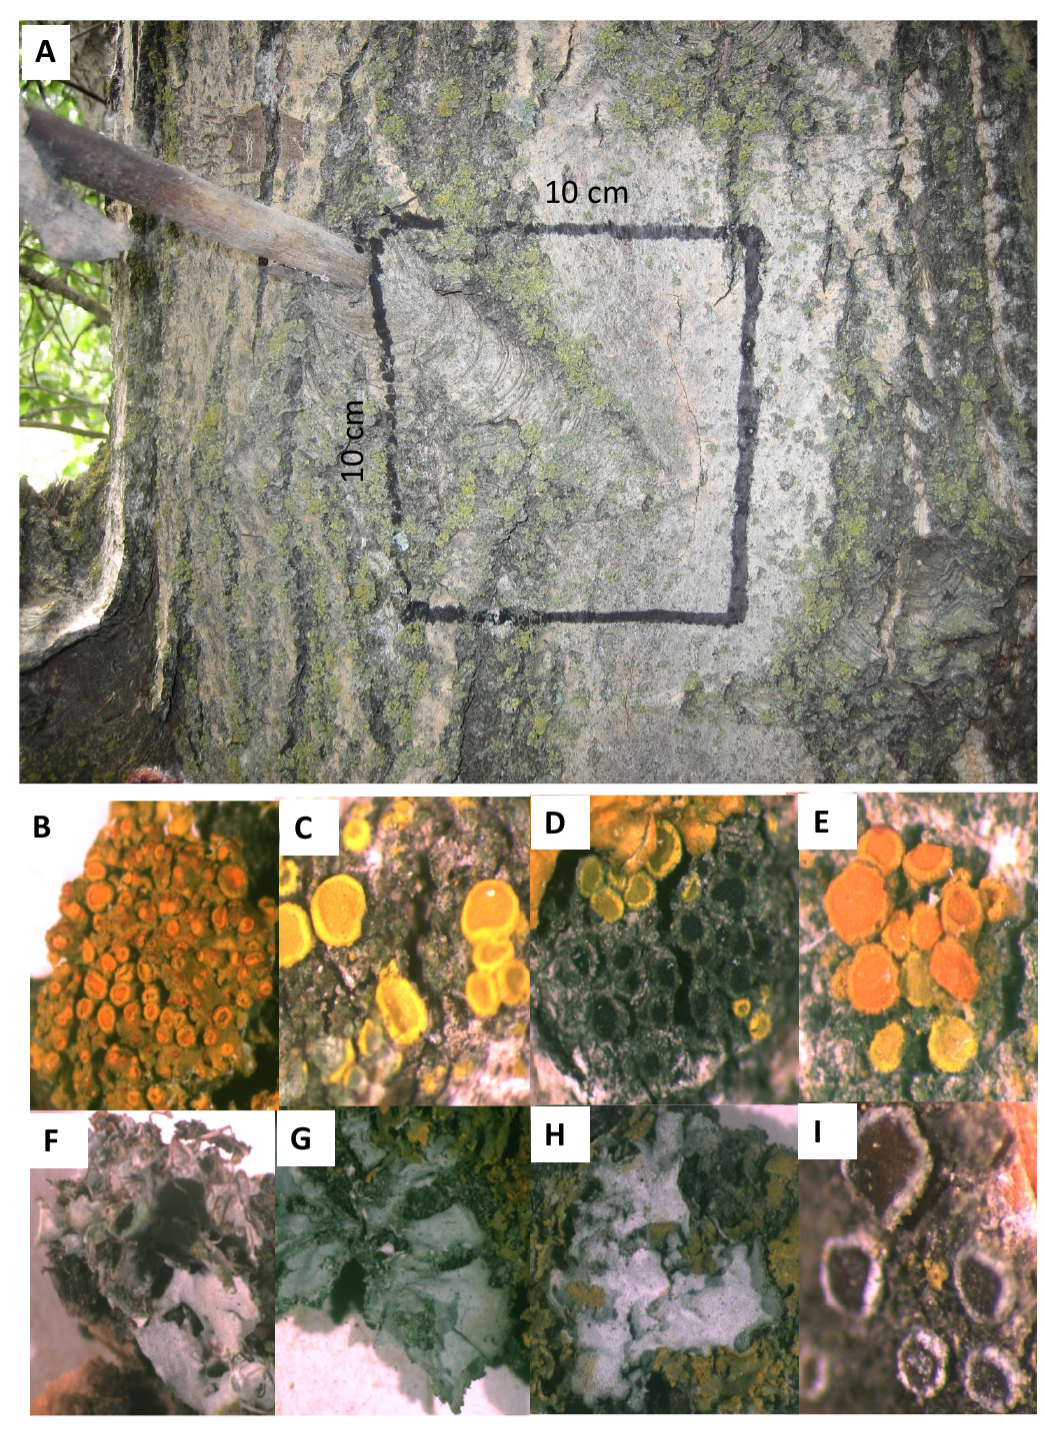
\includegraphics[width=0.90\linewidth]{figures/lcn_sampling.png}
\caption{The communities of bark lichens were observed in a common
  garden of replicated genotypes of narrowleaf cottonwood trees
  (\textit{P. angustifolia}) at the Ogden Nature Center (Ogden,
  UT). (A) Lichens were sampled within a fixed area (100 cm$^2$) on
  individual trees at two heights, 50cm and 95cm from the
  ground. (B-I) Close-up photos show the other lichen species
  observed, respectively:  \textit{Xanthomendoza montana},
  \textit{Candelariella subdeflexa}, \textit{Rinodina freyi},
  \textit{Athallia holocarpa}, \textit{Physcia adscendens},
  \textit{Physciella melanchra}, \textit{Physcia undulata} and
  \textit{Myriolecis hagenii}. Photo Credits: L.J. Lamit (B-D) and
  R. Reese Næsborg (E-I).}
\label{fig:lichen_sampling}
\end{figure}


\subsection*{Lichen Network Modeling}

For each tree, repeated observations of lichens were made in order to
construct replicated interaction networks for each genotype. We
conducted a modified sampling procedure originally developed by
\cite{Lamit2015a} with the addition that we quantified the presence of
lichens in the 1 cm$^2$ cells on individual trees of
\textit{P. angustifolia}. Unipartite networks were generated using the
conditional probabilities of each species pair, i.e., the probability
of observing one species given an observation of another species
$P(S_i | S_j)$, based on the method developed by \cite{Araujo2011}. To
calculate conditional probabilities, we quantified the individual
probabilities of species occurrences $P(S_i)$ and the joint
probability of co-occurrences $P(S_i, S_j)$ using the frequencies of
each species and their co-occurrences. We were then able to calculate
the conditional probabilities of each species pair as $P(S_i|S_j) =
\frac{P(S_i,S_j)}{P(S_j)}$, based on the axioms of probability. This
yielded a matrix that could possibly be asymmetric, i.e., $P(S_i|S_j)$
does not have to be equal to $P(S_j|S_i)$. Another important property
of this matrix is that the diagonal, $P(S_{i} | S_{i})$, was equal to
one for all species present and zero for species that were not
observed in any cell.

We then applied an analytical procedure to remove non-significant
links between species. This procedure determines if the joint
probability of a species pair (i.e., $P(S_i,S_j)$) is different from
zero (Fig.~\ref{fig:conet_method}).  Here, a confidence interval
$CI_{95\%}$ is calculated as as $CI_{95\%} = E[S_iS_j] * Z_{95\%} *
\sqrt{V(S_iS_j)}$, where the expected frequency of co-occurrences
E($S_iS_j$) is the total number of cells surveyed ($N$) times the
independent probabilities of each species $P(S_i) * P(S_j)$,
$Z_{95\%}$ is the Z-score for 95\% from a Z-distribution and the
expected variance of $E(S_iS_j)$ is the total number of cells times
the expected probability of $S_iS_j$ and its compliment (i.e.,
$V(S_iS_j) = N * E[P(S_i,S_j)] * (1 - E[P(S_i,S_j)])$). If the
observed number of co-occurrence falls outside of the confidence
interval, the joint probability $P(S_i,S_j)$ is determined to be equal
to the product of the individual probabilities (i.e., $P(S_i) \dot
P(S_j)$), and the conditional probability reduces to the individual
probability of that species $P(S_i)$. Therefore, unless the
co-occurrence of a species pair falls outside the confidence interval,
the probability that the observation of one species given the other is
no different than simply observing that species alone. This enables us
to remove links from a given network by re-scaling the resulting
conditional probabilities through subtraction of the individual
probabilities from the conditional probabilities (i.e., how different
the conditional probability is from the independent probability),
which makes any species with a non-significant conditional probability
zero.

The resulting matrix ($\mathbf{D} = D_{ij}$) can be interpreted as one
species' impact on another with zero being no effect and values less
than or greater than zero being negative and positive effects,
respectively. We will refer to $\mathbf{D}$ as a signed, weighted
interaction matrix. As such, $\mathbf{D}$ has the properties that it
can be asymmetric (i.e., $D_{ij}$ does not necessarily equal $D_{ji}$)
and it scales between -1 and 1, and, therefore, does not have the
mathematical properties of a probabilistic network
\citep{Poisot2016TheNetworks}. Also, as the method does not track
individuals within species and interactions such as competitive
exclusion or facilitation within species would result in the same
species being observed. Therefore, the results of intra-specific
interactions always results in the same species being observed and a
resulting $D_{ii} = 0$. In the context of these networks, asymmetry
and positive/negative valued connections are distinct
quantities. In-coming and out-going connections can be interpreted as
``influenced by'' and ``influenced'', respectively; while positive and
negative should be seen as one species increasing or decreasing,
respectively, the probability of another species' occurrence.

\begin{figure*}[ht]
\centering
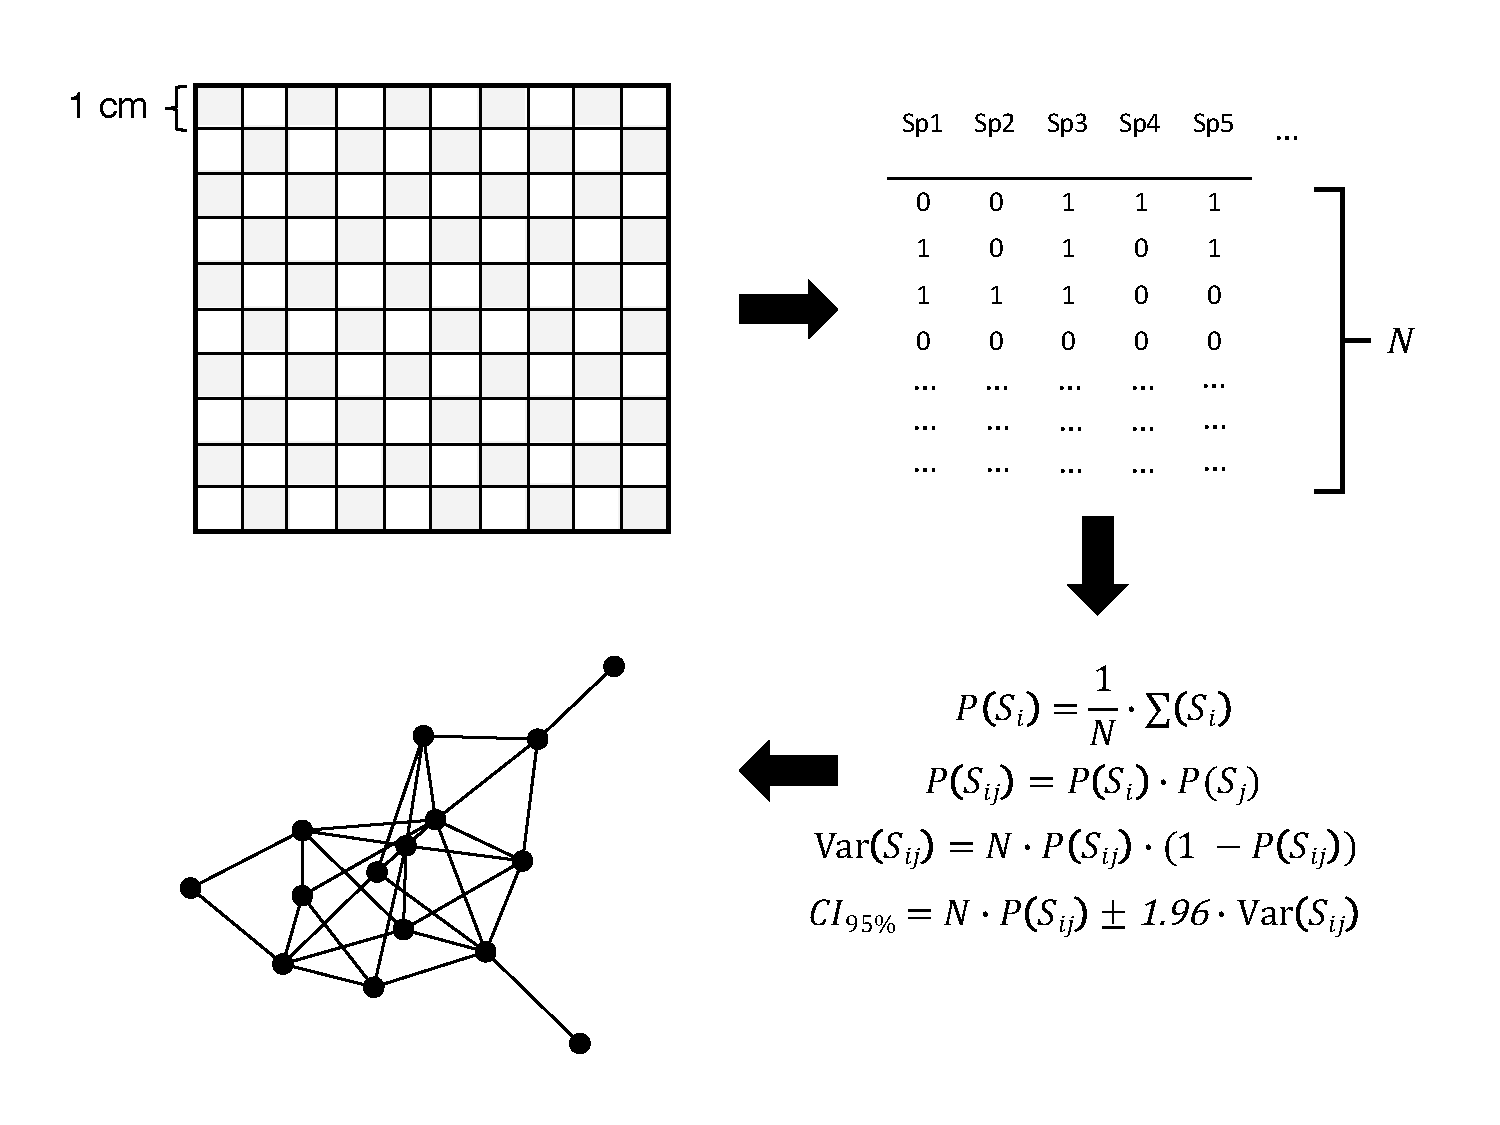
\includegraphics[width=\linewidth]{figures/lcn_araujo_method.pdf}
\caption{Lichen interaction networks were constructed by conducting
  field observations in 1 cm$^2$ cells within a 100 cm$^2$ grid on each
  tree using a checkerboard pattern (grey cells). Thus, a set of $N$
  total cell observations were recorded for each tree with the
  presence or absence of each species recorded for each cell. Applying
  the probability-based network modeling method adapted from
  \citep{Araujo2011}, we calculated the conditional probabilities,
  $P(S_i|S_j)$, for all species pairs and removed (i.e., set equal to
  zero) species pairs whose joint probabilities, $P(S_i S_j)$, were
  not significant using a confidence interval based comparison of
  their observed co-occurrence frequency, $S_iS_j$, to that expected
  due to chance alone, $E[P(S_iS_j)] = P(S_i) P(S_j)$, and
  $P(S_i|S_j)$ reduces to $P(S_i)$, the observed individual
  probability of species $S_i$.}
\label{fig:conet_method}
\end{figure*}


\subsection*{Analyses, Software and Data}

To quantify the structural variation of lichen networks we calculated
several metrics at both the level of node and whole networks. Although
there are many other metrics, for the sake of simplicity we focus on a
subset that represent the primary interesting features of network
structure, see \cite{Lau2017a}. We calculated the number of
interactions or ``links'' in each network (degree), which provides a
measure of the size of the network \citep{Lau2016afix,
  Borrett2014EnaR:Analysis}. We also calculated the centralization of
each network using Freeman's centrality, which measures the evenness
of the distribution of interactions among the species in the network,
using the \texttt{sna} package \citep{sna}. In a network with low
centralization species have similar strengths and numbers of
interactions. A network with high centralization tends to have one or
small number of species that interact with other species. We used a
related function to calculate the centrality of each species (i.e.,
node level centrality) in each network as well. To calculate separate
metrics for positive and negative links, as the networks contained not
only positive and negative connections but also directional
connections (both in-coming and out-going), we calculated the same
network metrics for all combinations of these types of connections
using recently developed methods for signed, weighted and directed
networks \citep{Everett2014NetworksTies} using the \texttt{signnet}
package \citep{signnet}.

We used a combination of parametric and non-parametric, permutation
based frequentist statistical analyses to test for the effects of
genetic variation on lichen communities and their interaction
networks. To assess the effect of genotype on traits as univariate
response variables (including the metrics of network structure), we
used additive, random effects models with Restricted Maximum
Likelihood (REML) conducted in R via the \texttt{lme4} and
\texttt{RLRsim} packages \citep{lme4, RLRsim}. To conform to test
assumptions, traits were root transformed with the exception of
condensed tannin concentration and carbon-nitrogen ratio, which were
rank and log$_{10}$ transformed, respectivley. Differences in node
level centrality among species was tested using ANOVA and Tukey-HSD
multiple comparison tests. Correlations among trait variables and
network metrics were quantified and tested using linear correlations
of Pearson's $r$. For multivariate response variables, such as lichen
community composition and network structure, we used distance based
multivariate statistical approaches. To quantify the similarity of
lichen networks among individual trees, we calculated the pairwise
Euclidean distance of the $\mathbf{D}$ interaction matrices among all
trees \citep{Newman2010}. To test for the effects of genotype and
other predictor variables on network similarity we conducted
Permutational Analysis of Variance (PERMANOVA) with \texttt{vegan}
\citep{vegan}. For visualization of multivariate patterns, we used
Non-metric Multi-Dimensional Scaling (NMDS) \citep{ecodist} to produce
dimensionally reduced ordinations of these multi-variate responses and
fitted vectors for continuous predictor variables to the ordinated
values \citep{vegan}. Using random initial configurations with a
maximum of 500 iterations and a change in stress threshold of less
than 10$^{-12}$. This was repeated for one to four dimension
configurations, and the configuration with the lowest dimensionality
and unexplained variation less than 10\% was selected. For all tests
where genotype was used as a predictor, we quantified the heritability
of the response variable. Because the trees in the garden were clonal
replicates of each genotype, we calculated broad-sense heritability,
which is the genotypic variance divided by the total phenotypic
variance \citep{Conner2004ATextbook}, which can be interpreted as a
measure of the phenotypic variance due to genotypic variation. All
analyses were conducted using R version 4.0.2 \citep{R2020}. Code and
data for the project are openly available as a reproducible workflow
using \texttt{drake} \citep{drake}, which is archived via Zenodo
\url{zenodo.com/doiXXXXXX}.

\begin{figure}[ht]
\centering
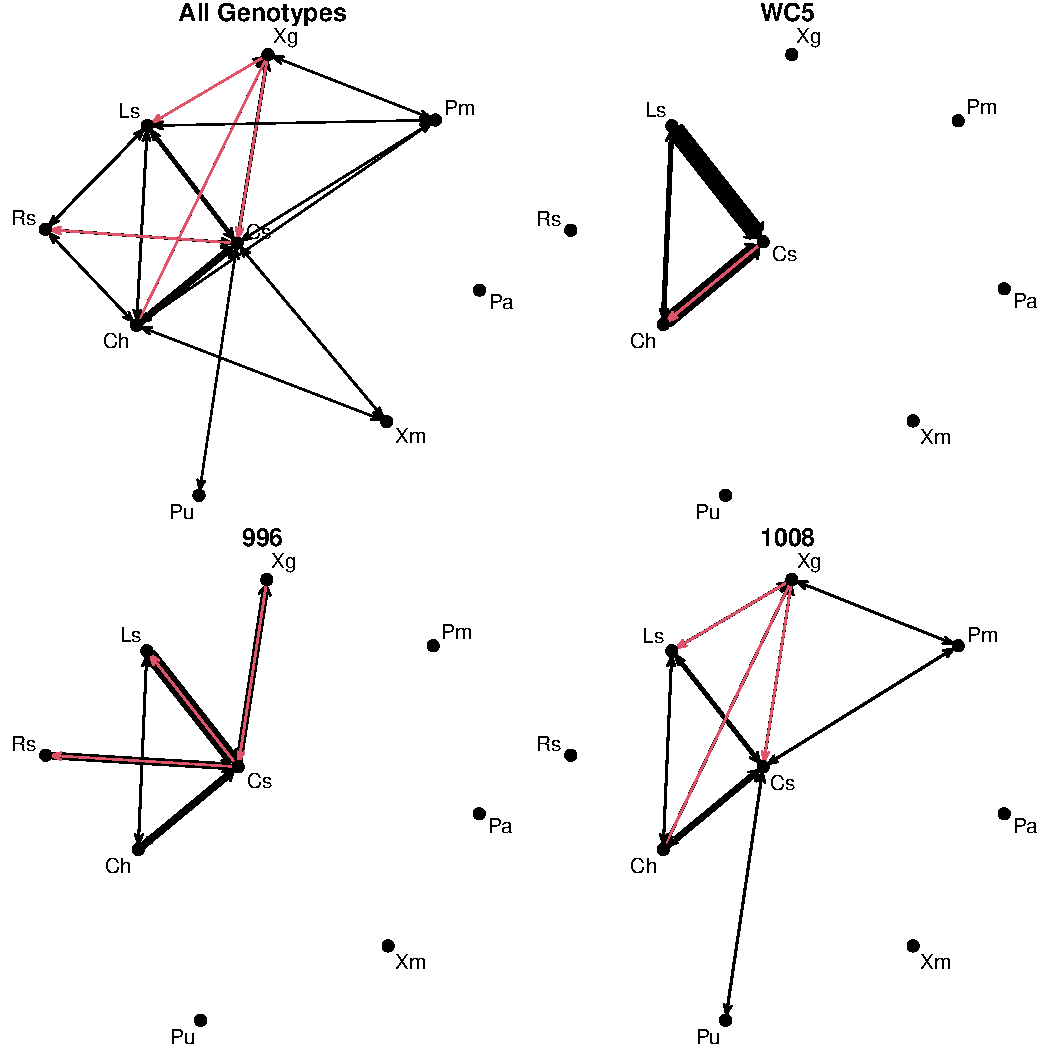
\includegraphics[width=\linewidth]{figures/cn_onc.pdf}
\caption{Lichen networks varied in structure among tree
  genotypes. Network diagrams of the mean lichen interaction matrices
  averaged for all trees and for illustrative genotypes (996, WC5 and
  1008) showing a range of interaction network
  structure. Directionality (arrowheads) and sign (red = negative,
  black = positive) of interactions are shown as edges between
  species, which are scaled by their magnitude.  Species names are
  abbreviated by the first letter of the genus and specific epithet:
  Ah = \textit{Athallia holocarpa}, Cs = \textit{Candelariella
    subdeflexa}, Mh = \textit{Myriolecis hagenii}, Rf =
  \textit{Rinodina freyi}, Pa = \textit{Physcia adscendens}, Pm =
  \textit{Physciella melanchra}, Pu = \textit{Physcia undulata}, Xg =
  \textit{Xanthomendoza galericulata}, Xm = \textit{Xanthomendoza
    montana}. The sign of the interaction is indicative of greater
  (positive) or lesser (negative) paired occurrences than expected
  relative to the overall frequency of occurrence of each
  species. Ecologically, the links in the network are likely the
  product of multiple types of interactions (e.g. mutualism,
  parasitism, competition, facilitation) that could vary over both
  space and time.}
\label{fig:geno_nets}
\end{figure}

\section*{Results}

In support of our first hypotheses, we found that tree genotype
influenced lichen network structure and that multiple lichen network
metrics were heritable. Tree genotype significantly predicted the
structural similarity of lichen networks and, overall, network-level
metrics responded significantly to tree genotype, including network
degree and centralization including both in-coming and out-going links
or when separated into in-coming only or out-going only
(Table~\ref{tab:h2_net}, Fig.~\ref{fig:h2_plot}).  Metrics including
only positive links also showed a significant effect of tree genotype,
including positive degree and positive in-going centralization.
Metrics calculated with negative links were not significant, including
degree (negative) and both in-coming (negative) and out-going
centralization (negative).

\begin{figure*}[ht]
\centering
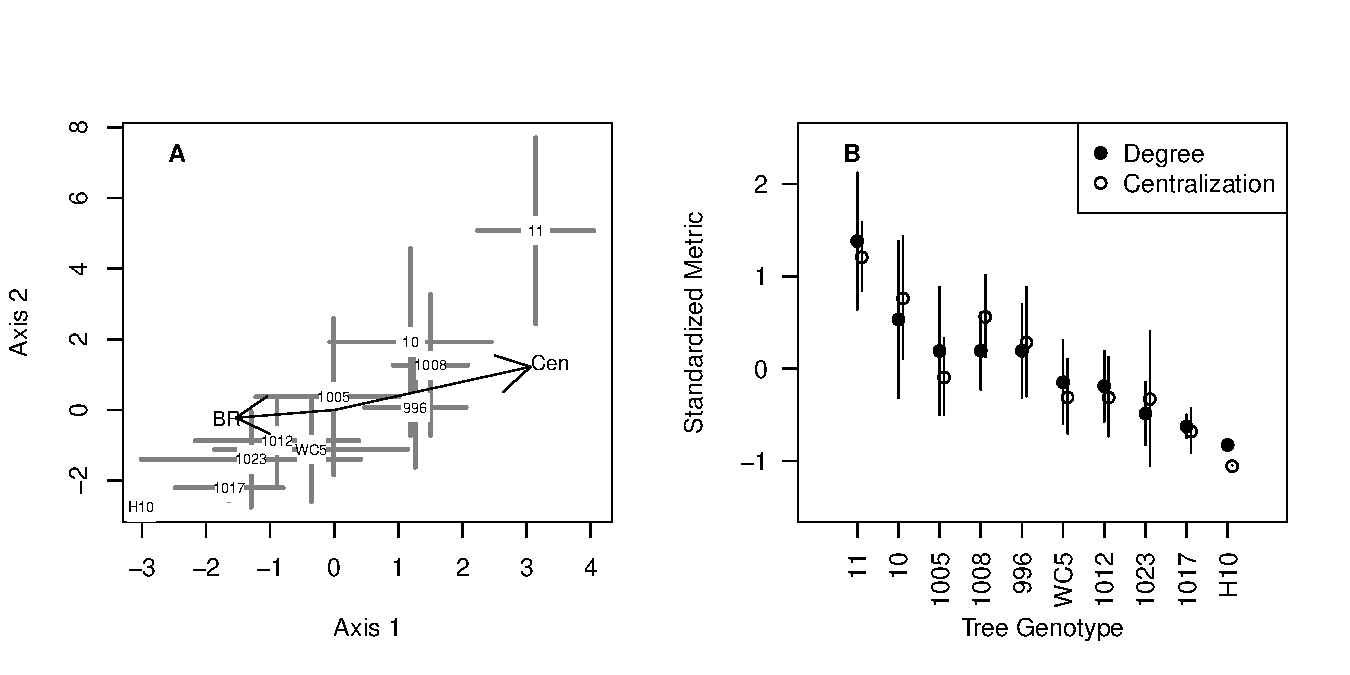
\includegraphics[width=\linewidth]{figures/h2_plot.pdf}
\caption{The similarity of lichen networks varied among tree
  genotypes. A. The plot shows genotype centroids of NMDS ordinated
  (R$^2$ = 0.999, stress = 0.008) lichen network similarity ($\pm$ 1
  S.E.). Genotype centroids that are closer together tend to have more
  similar lichen network structure. Arrows showing the direction
  (arrowhead) and magnitude (length) of the vectors of correlation
  between bark roughness (\textbf{BR}) and network centralization
  (\textbf{Cen}) and the ordinated networks. B. Plot showing
  the standardized ($\frac{x - \bar{x}}{\sigma}$) means ($\pm$ 1 S.E.)
  for the two of the genetically based lichen network metrics: overall
  degree (i.e., total number of links) and centralization, which is a
  measure of the dominance of one species in the network.}
\label{fig:h2_plot}
\end{figure*}

% latex table generated in R 3.6.3 by xtable 1.8-4 package
% Wed Dec  2 18:23:39 2020
\begin{table}[ht]
\centering
\begin{tabular}{rrrrr}
  \hline
Response & df & $RLRT$ & $H^2$ & p-value \\ 
  \hline
Lichen Network Similarity & 9 & 3.5821 & 0.41 & 0.0537 \\ 
  Degree & 9 & 3.5175 & 0.32 & 0.0255 \\ 
  Degree (positive) & 9 & 3.6925 & 0.32 & 0.0229 \\ 
  Degree (negative) & 9 & 0.0327 & 0.03 & 0.3859 \\ 
  Centralization & 9 & 4.0444 & 0.33 & 0.0184 \\ 
  Centralization In-Degree & 9 & 4.4812 & 0.35 & 0.0142 \\ 
  Centralization In-Degree (positive) & 9 & 3.9852 & 0.33 & 0.0190 \\ 
  Centralization In-Degree (negative) & 9 & 0.3304 & 0.11 & 0.2508 \\ 
  Centralization Out-Degree & 9 & 3.8615 & 0.32 & 0.0205 \\ 
  Centralization Out-Degree (positive) & 9 & 3.5585 & 0.31 & 0.0248 \\ 
  Centralization Out-Degree (negative) & 9 & 0.0862 & 0.05 & 0.3446 \\ 
   \hline
\end{tabular}
\caption{Genotypic effects on the associated lichen network structure. $RLRT$ is the statistic from the restricted likelihood ratio tests.} 
\label{tab:h2_net}
\end{table}


The genetic response of network centralization was driven by variation
in \textit{Athallia holocarpa}. Centrality varied significantly among
species ($F_{8, 324}$ = 7.99, $R^2$ = 0.16, \textit{p-value} $<$
0.0001). \textit{Athallia holocarpa} was the main species
to exhibit a significant response to tree genotype in terms of
positive centrality for both the in-coming (\textit{RLRT} = 3.61,
$H^2$ = 0.32, \textit{p-value} = 0.0240) and out-going (\textit{RLRT}
= 3.13, $H^2$ = 0.30, \textit{p-value} = 0.0327) perspectives, but not
for either negative centrality metrics in-coming (\textit{RLRT} = 0,
$H^2$ = 0, \textit{p-value} = 1) or out-going (\textit{RLRT} = 0,
$H^2$ = 0, \textit{p-value} = 0.4543). None of the other species'
centralities showed a genotypic response (Supporting Information,
Fig. 2) with the exception of \textit{X. montana} (\textit{RLRT} =
2.92, $H^2$ = 0.32, \textit{p-value} = 0.0375); however, the
centrality of \textit{X. montana} was much lower overall relative to
\textit{A. holocarpa} and the variation in \textit{X. montana}
centrality was restricted to two genotypes
(Fig.~\ref{fig:geno_sppcen}).



\begin{figure*}[ht]
\centering
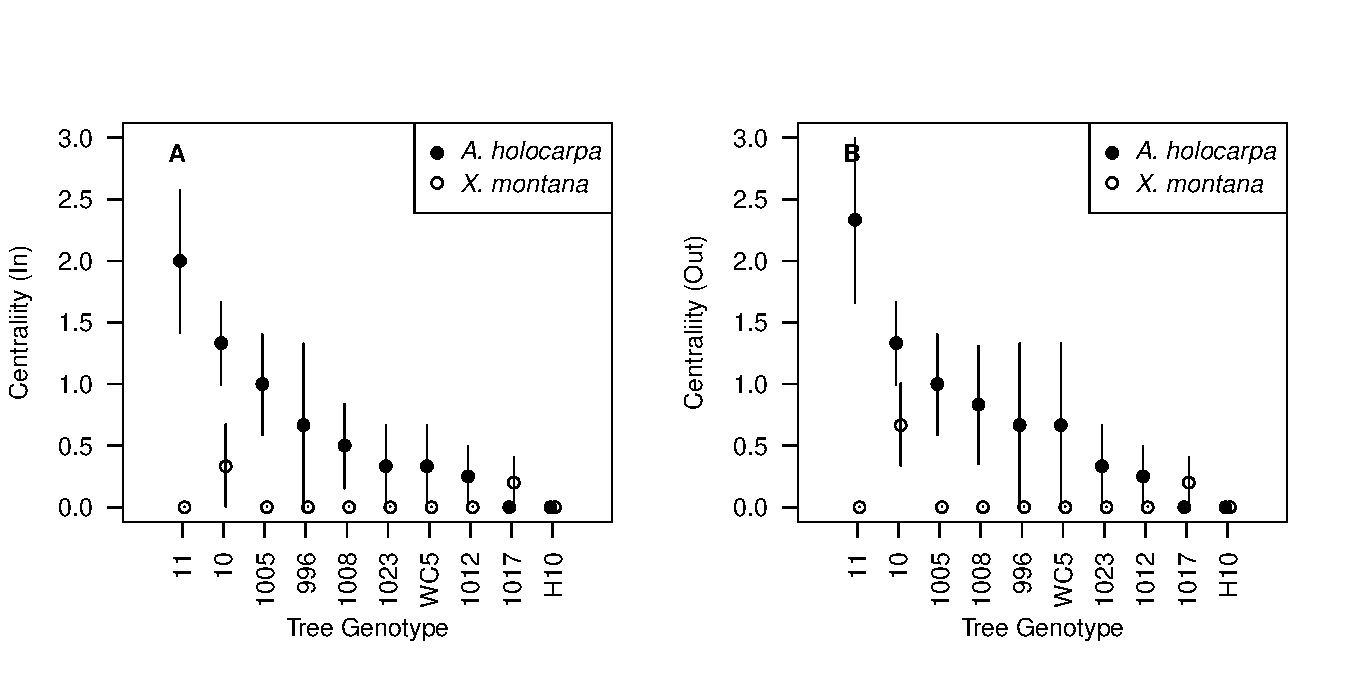
\includegraphics[width=\linewidth]{figures/geno_sppcen.pdf}
\caption{Dot-plots showing the mean (dot) and $\pm$ 1 SE of in-degree
  (A) and out-degree (B) centrality for two species,
  \textit{A. holocarpa} and \textit{X. montana}. \textit{Athallia
    holocarpa} centrality was highly variable among
  genotypes. \textit{Xanthomendoza montana} centrality, both in- and
  out-degree, was only non-zero for two genotypes, and only out-degree
  centrality displayed a significant response to genotype.}
\label{fig:geno_sppcen}
\end{figure*}

In support of our second hypothesis, analysis of trait covariation
revealed that genotype indirectly influenced lichen network
centralization via genetically based variation in bark roughness. The
percent cover of rough bark (\textit{RLRT} = 4.8526, $H^2$ = 0.3221,
\textit{p-value} = 0.0113) and condensed tannins (\textit{RLRT} =
3.0522, $H^2$ = 0.3205, \textit{p-value} = 0.0343) both displayed
significant responses to tree genotype. None of the other bark traits,
pH (\textit{RLRT} = 0.00, $H^2$ = 0.00, \textit{p-value} = 1.0000) or
carbon-nitrogen ratio (\textit{RLRT} = 0.0000, $H^2$ = 0.0000,
\textit{p-value} = 1.0000), showed a significant response to tree
genotype and none other than bark roughness was correlated with
network similarity (Table~\ref{tab:cn_trait_perm}); therefore, we
focused our subsequent analyses on the indirect effect of genotype on
lichen network structure via bark roughness. We found that bark
roughness was significantly correlated with network similarity and
other lichen network metrics, including negative correlations with
overall network degree ($df$ = 35, $t$ = -2.13, $r$ = -0.34,
\textit{p-value} = 0.04) and centralization ($df$ = 35, $t$ = -2.52,
$r$ = -0.39, \textit{p-value} = 0.02). In other words, trees with more
similar levels of bark roughness tended to have lichen interaction
networks with similar structure. To quantify the genetic bases of this
effect of bark roughness on network structure, we used the residual
values from regressions of network degree and centralization in tests
of the effect of tree genotype and found no significant effect of tree
genotype for either degree (\textit{RLRT} = 0.00, $H^2$ = 0.00,
\textit{p-value} = 1.0000) or centralization (\textit{RLRT} = 0.00,
$H^2$ = 0.00, \textit{p-value} = 1.0000), suggesting that the observed
relationship between bark roughness and lichen network structure was
largely genetically based (Fig.~\ref{fig:br_net}).

% latex table generated in R 4.0.2 by xtable 1.8-4 package
% Mon Feb  1 17:29:25 2021
\begin{table}[ht]
\centering
\begin{tabular}{rrrrrr}
  \hline
 & df & SS & R2 & Pseudo-F & p-value \\ 
  \hline
Bark Roughness & 1 & 20850.09 & 0.26 & 12.9234 & 0.0101 \\ 
  Condensed Tannins & 1 & 5993.66 & 0.07 & 3.7150 & 0.0813 \\ 
  pH & 1 & 1273.19 & 0.02 & 0.7892 & 0.3712 \\ 
  Carbon:Nitrogen Ratio & 1 & 3896.18 & 0.05 & 2.4150 & 0.1890 \\ 
  Residual & 32 & 51627.33 & 0.64 &  &  \\ 
  Total & 36 & 80993.59 & 1.00 &  &  \\ 
   \hline
\end{tabular}
\caption{PERMANOVA Pseudo-F Table of lichen network similarity response to bark traits.} 
\label{tab:cn_trait_perm}
\end{table}


\begin{figure*}[ht]
\centering
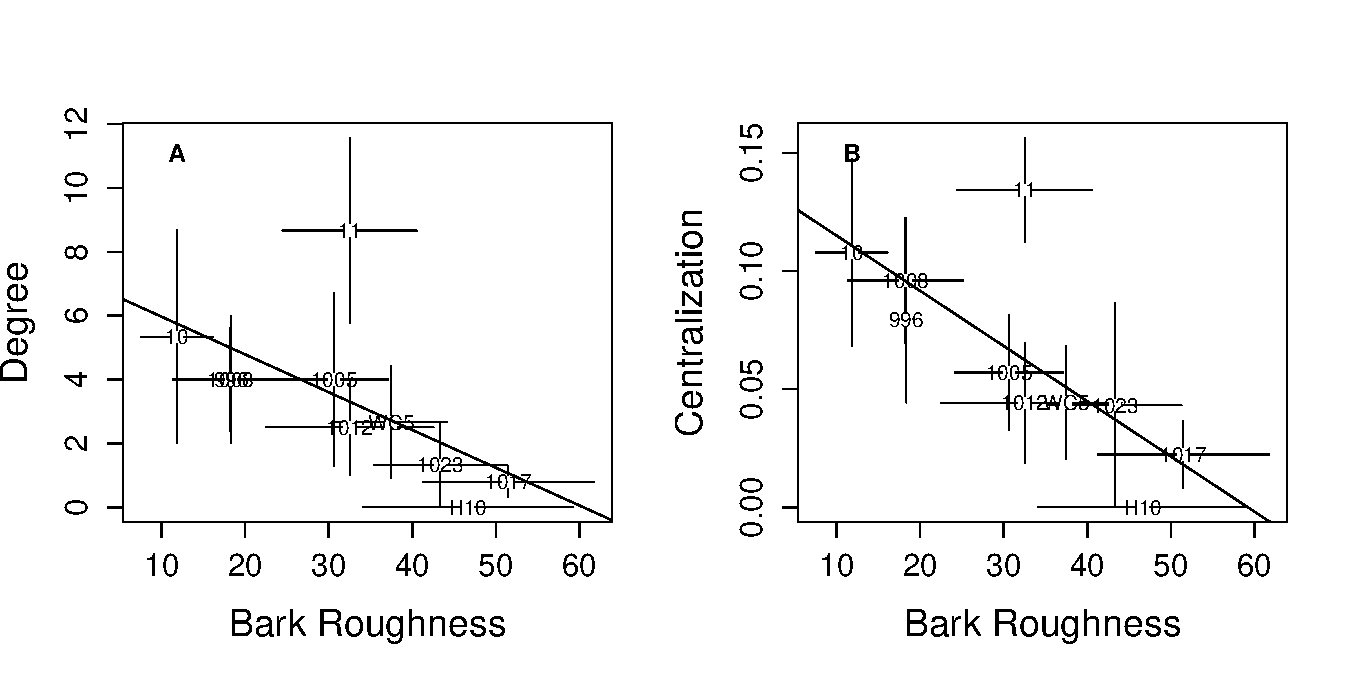
\includegraphics[width=\linewidth]{figures/br_net.pdf}
\caption{Bivariate plots of the negative relationship between bark
  roughness and two network metrics: A) degree and B)
  centralization. Each plot displays the genotype mean ($\pm$ 1 S.E)
  for both variables and a least-squares regression line calculated
  using the genotype means. Generally, as roughness increased the
  number of interactions (degree) and dominance of
  those interactions (centralization) decreased.}
\label{fig:br_net}
\end{figure*}


\section*{Discussion}

Subsection changes proposed by Tom

\begin{itemize}
\item Current
  \begin{itemize}
  \item Implications of Ecological Network Heritability
  \item Evolution and Genetically Based Network Structure
  \item Conclusion
  \end{itemize}
\item TGW
  \begin{itemize}
  \item Importance of Network Heritability
  \item Networks and Levels of Seletion in Community Evolution
  \item Conclusions
  \end{itemize}
\end{itemize}


\textbf{START TGW}

DISCUSSION (omitted the intro para and moved to conclusions)

Importance of Network Heritability

Although previous studies have examined aspects of networks, such as
trophic
340 complexity (Barbour et al., 2016) and forest stand-level
interaction network structure
341 (Lau et al., 2016b; Keith et al., 2017), this is the first study
that we are aware of to
342 examine the heritability of network structure with replicated
networks at the genotype
343 scale. Previous work in the evolution of ecological networks have
primarily focused on
344 macro-evolutionary dynamics (Rezende et al., 2007; Weber et al.,
2017; Valverde et al.,
345 2018; Harmon et al., 2019) or have been simulation based
individual-level models that
346 integrate intraspecific variation to the species level (Maliet et
al., 2020), even though
347 recent syntheses have pointed to the importance of processes
operating across scales of
348 organization (Guimara˜es, 2020). There are two important
functional ramifications of
349 genetically based variation in network structure.
            First,
            Second,
            Furthermore,


Networks and Levels of Selection in Community Evolution

\textbf{START MKL}

Per general systems theory, ecosystems are generally:

\begin{itemize}
\item self-organizing: an effect is its own cause (autocatalytic, cycles)
\item holarchic: spatially and temporally nested, hierarchical  sub-systems
\item open: energy and matter passes across the system boundary
\end{itemize}

The holarchic nature provides a means for superior systems, i.e. the
foundation species, to influence the sub-systems, i.e. the lichen
networks, by altering the success and survival of individuals and/or
their traits, both of which can alter the structure of interaction
networks.

Evolutionarily, frequencies of traits (or genotypes) can increase or
decrease in their moment of central tendancy, spread, and/or
kurtosis. 

\textbf{END MKL}

Multilevel selection theory argues that selection can occur
simultaneously at individual, group and community levels and the
demonstration of evolution at any scale requires demonstrating three
key elements (review by Whitham et al. 2020). The community networks
in our study are based upon the interactions of the lichen community
in which the differential survival and performance of individual tree
genotypes will simultaneously result in selection occurring on the
lichen community it supports. (We could introduce holobiont theory
here). First, for selection to occur at the community level, there
must be variation in the structure (composition,
426 abundance, species interactions, diversity, networks) of
communities across the tree land427
scape. Second, these differences must be genetically based and
heritable in which
428 community structure is passed from one tree generation to the
next. For example, numerous
429 studies show that related individuals tend to support the same
communities of insects
430 and microbes, and ecosystem processes of biodiversity, nutrient
cycling and stabil431
ity, whereas unrelated individuals support more different communities
and ecosystem
432 processes. Importantly, the current
433 study shows that networks are also heritable traits that greatly
increases its utility as a
434 community phenotype that selection can act upon. Third, selection
must act on these
435 differences to favor some communities over others leading to
change over time

(i.e.,
436 community evolution). Since our findings show genetic variation in
lichen networks and show that lichen networks are heritable, future
studies should evaluate how networks might change over time in
response
438 to an invasive species, climate change, or some other agent of
selection. For example, in this study, when a tree dies due to
drought, its community network of interacting lichens is selected
against, while those networks of other trees that survive persist. 
Thus, if drought related mortality is non-random as shown by Sthultz
et al. (2009), network structure can evolve via selection acting on
whole communities.

439                  In the present study, intraspecific, genotypic
diversity in the heritable bark traits of individual trees appear to
be a major causal factor resulting in the creation of lichen
meta-communities ….

Conclusions – I think this intro to the Discussion is a better
conclusion section could be merged with the your old conclusions
section.  I suggest that it be more focused with key numbered points.
We found support for both of our hypotheses. First, tree genotype
influenced the network
323 structure of lichen communities associated with narrowleaf
cottonwoods in a riparian
324 forest ecosystem. Network similarity and metrics of network
structure tended to be more
325 similar on trees of the same genotype. Generally, this genetic
effect was manifested
326 in positive interactions and largely driven by A. holocarpa. (Not
sure what the broader point of this sentence on A. holocarpa is as it
appears to weaken a community perspective??  Need to clarify.  Second,
the genetically
327 based trait, bark roughness, was observed to affect network
variation, largely via shifts
328 in positive in-coming and out-going interactions. Chemistry
traits, whether genetically
329 based (e.g., tannin concentration) or not, were not significantly
correlated with lichen

330 network structure. Bark roughness has been demonstrated previously
to be under strong
331 genetic control (Bdeir et al., 2017), and bark roughness has also
been shown to be an
332 important tree trait influencing bark lichens (Lamit et al.,
2015b); however this is the
333 first demonstration of a link from genetics to lichen network
structure. As such, these
334 results have important implications for the influence of
genetically based variation in
335 ecosystems with networks of interacting species.



\textbf{END TGW}



We found support for both of our hypotheses. First, tree genotype
influenced the network structure of lichen communities associated with
narrowleaf cottonwoods in a riparian forest ecosystem. Network
similarity and metrics of network structure tended to be more similar
on trees of the same genotype. Generally, this genetic effect was
manifested in positive interactions and largely driven by
\textit{A. holocarpa}. Second, the genetically based trait, bark
roughness, was observed to affect network variation, largely via
shifts in positive in-coming and out-going interactions. Chemistry
traits, whether genetically based (e.g., tannin concentration) or not,
were not significantly correlated with lichen network structure. Bark
roughness has been demonstrated previously to be under strong genetic
control \citep{Bdeir2017}, and bark roughness has also been shown to
be an important tree trait influencing bark lichens
\citep{Lamit2015a}; however this is the first demonstration of a link
from genetics to lichen network structure.  As such, these results
have important implications for the influence of genetically based
variation in ecosystems with networks of interacting species.


\subsection*{Implications of Ecological Network Heritability}

Significant heritability of lichen interaction network structure is in
line with the genetic similarity rule, in which networks observed on
trees of the same genotype tended to be structurally similar. Although
previous studies have examined aspects of networks, such as trophic
complexity \citep{Barbour2016GeneticComplexity} and forest stand-level
interaction network structure \citep{Lau2016GenotypicEvolution,
  Keith2017}, this is the first study that we are aware of to examine
the heritability of network structure with replicated networks at the
genotype scale. Previous work in the evolution of ecological networks
have primarily focused on macro-evolutionary dynamics
\citep{Rezende2007, Weber2017EvolutionMacroevolution,
  Valverde2018TheSpandrel, Harmon2019DetectingInteractions} or have
been simulation based individual-level models that integrate
intraspecific variation to the species level
\citep{Maliet2020AnNetworks}, even though recent syntheses have
pointed to the importance of processes operating across scales of
organization \citep{Guimaraes2020TheOrganization}. There are two
important functional ramifications of genetically based variation in
network structure.

First, heritability of network structure suggests that some amount of
interaction network complexity is determined and therefore could be
predicted by genetic identity. Variation in space and time create
variation in ecological networks that influences evolutionary dynamics
via shifts in ecological dynamics, such as population demographics
\citep{Guimaraes2020TheOrganization}. Given that ecosystems are
comprised of hundreds and thousands of species, each having a
multitude of interactions, the potential to find traction for making
predictions in the context of ecological, let alone evolutionary,
dynamics seems daunting. The promise of predictability lies in the
presence of asymmetries in ecosystems, such as hierarchy created by
foundation species via differences in body size and/or life-history
strategies \citep{Ellison2005}. The second is that heritability (i.e.,
genetic determination) means that there is structure in the spatial or
temporal variation that is created by individuals of foundation
species whose traits are in part determined by underlying trait
differences. Although this variation is inherently a function of both
genetic and environmental effects \citep{Conner2004ATextbook}, the
community and network-level effects are also a function of the scale
of the interaction \citep{Shuster2006COMMUNITYSTRUCTURE}.


Second, even if the composition of the communities is the same among
individuals and genotypes, interactions may not be. We didn't observe
compositional differences using the same data from which the lichen
networks were derived. If we only had our composition dataset from
this study, we would have concluded no response of the lichen
community to tree genotype, even though the underlying interactions
among lichen species does vary among genotypes. As such differences in
network structure could occur without observable differences in
species richness or community composition, which have been the primary
focus of almost all previous community genetics studies
\citep{DesRoches2018TheVariation}. Community composition of lichens
has previously been observed to be different among tree genotypes in
the same experimental garden \citep{Lamit2011, Lamit2015a}. The
different results observed in the present study is likely a result of
differences in lichen quantification and the tree genotypes observed
leading to overall higher abundances of observed lichens to assure the
possibility of observing lichen interactions. The previous study used
a visual percent cover estimation, unlike the current study, which
observed lichens at the scale of 1 cm$^2$ cells, which could
over-estimate cover depending on the frequency at which actual thallus
size was less than 1 cm$^2$, as well as both the northern and southern
aspects of each tree. These differences do not negate the findings of
either study. The present study's finding of differences in network
structure without significant compositional differences points to the
importance of quantifying how network structure changes in response to
genetic variation in order to fully understand evolutionary dynamics
in complex communities. Having not observed a compositional effect of
tree genotype without measuring the network structure could lead to
the conclusion of no genetic effect on the community, even though
differences in network structure are leading to altered, local
evolutionary dynamics. It is possible that these underlying
differences in interactions among lichens could lead to differences in
community composition at a future point in time via their effects on
species abundances \citep{Shuster2006COMMUNITYSTRUCTURE}; however,
this is not needed for evolutionary dynamics to occur via selection
that leads to shifts in trait distributions without shifting species
abundance distributions, which is possible under stabilizing,
disruptive and directional selection \citep{Conner2004ATextbook}, so
long as the relative abundances of each species is imperceptibly
changed. Thus, it is imperative that further community genetics
research assess or at least be aware of the potential effects of
variation in interactions and not just observe species abundances,
otherwise community level genetic effects may be underestimated,
especially when cumulative interaction effects are taken into account
\citep{Borrett2007FunctionalProliferation, Borrett2010}.

Furthermore, the demonstration of the heritability of interaction
networks, without significant differences in community composition,
provides clear empirical evidence that variation in network structure
points to the need to expand IIGEs to encompass the structure of
interaction networks. Although IIGE theory provides a quantitative
framework within which to approach evolutionary theory at higher
levels of biological organization (from populations to communities and
ecosystems), this theory has focused on modeling the strong effects of
foundation species \citep{Shuster2006COMMUNITYSTRUCTURE, Whitham2012,
  Whitham2020IntraspecificEvolution} and has not yet integrated
developments from the ecological or evolutionary network theory
literature. Thus, it has not developed a way to examine complex
interactions among species; however, previous studies have
demonstrated this network context is likely to be important, as
altering the structure of interaction networks provides a means for
genetic effects to be dampened or magnified within the system of
interacting species \citep{Smith2011, Keith2017}. Although such a
synthesis necessitates a much greater effort than can be afforded in
this paper, it is possible to point to several productive pathways
forward. In terms of interaction networks, foundation species are
relatively central within the system of interactions, that is their
direct and/or indirect effects are greater than other species. So,
when the more centralized (foundation) species have genetically based
interactions, genetic effects will tend to be propagated and possibly
magnified in the community. Here, we found that even though more
abundant or more centralized (i.e., ``important'') species were
present in the community, their effects were not the singularly
responding to genetic effects, rather the similarity of the whole
network depending on interactions among multiple species. Considering
the impact of network structure would be a productive path forward for
the theoretical development and application of the IIGE concept.


\subsection*{Evolution and Genetically Based Network Structure}

The demonstration of evolution at any scale of biological organization
requires demonstrating three key elements \citep{Conner2004ATextbook},
which have been extended to higher levels of ecological organization
\citep{Whitham2003, Whitham2006a, Whitham2020} . First, there must be
variation in the structure (composition, abundance, species
interactions, diversity, interaction network structure) of
communities. Second, these differences must be genetically based and
heritable in which community structure is passed from one generation
to the next. For example, numerous studies show that related
individuals tend to support the same communities of insects and
microbes, and ecosystem processes of biodiversity, nutrient cycling
and stability, whereas unrelated individuals support more different
communities and ecosystem processes \citep{Bangert2006, Bangert2008a,
  Whitham2020IntraspecificEvolution}. Importantly, the current study
shows that networks are also heritable traits that greatly increases
its utility as a community phenotype that selection can act
upon. Third, selection must act on these differences to favor some
communities over others leading to change over time (i.e., community
evolution). Since our findings show that networks are heritable,
another metric of community evolution is showing how networks change
over time in response to an invasive species, climate change, or some
other agent of selection.

Intra-specific, genotypic diversity among cottonwood trees is creating
meta-communities of lichens on individual trees that form interaction
modules with different dynamics. When communities are comprised of
individuals whose habitat is primarily determined by another organism,
these communities inherently form modules within the larger ecosystem,
as they tend to interact more with each other than with other
individuals \citep{Lau2017a}. Our study demonstrates that the
environmental differences determined by the genetic variation within a
single tree species can not only impact community composition, as
repeatedly demonstrated in other community genetics studies
\citep{Whitham2006a, DesRoches2018TheVariation}, but also shape the
structure of interactions among individuals. Some network structures
are likely to be more stable, either in response to disturbance or via
self-organized dynamics. For example, centralized networks, although
more efficient, are theorized to be more susceptible to targeted
``attacks'' in the terminology of defense networks. As mentioned
previously, one class of networks that are theorized to have
amplifying effects on networks have centralized "star" shapes with one
or a few species at the center and radiating interactions out from the
central core \citep{Lleberman2005EvolutionaryGraphs}. This is
structurally what we have observed with the networks that tend to
occur on some of the genotypes in our study, i.e., the more
centralized networks. It is likely that these networks could function
as hot-spots of evolutionary dynamics resulting from the amplifying
effect the centralized network structure found on that tree genotype,
as multiple studies have found significant impacts of the removal of
foundation species in different systems \citep{Keith2017,
  DesRoches2018TheVariation}.


Ecological network studies have focused on asymmetry and the
quantification of its structure in communities. The impacts of
asymmetry on evolution from community dynamics have primarily produced
qualitative discussion \citep{Bascompte2006, Diaz-Castelazo2010,
  Guimaraes2011, Thompson2013}. More specific predictions can be found
in applications of evolutionary game theory, and although developed at
the population scale, such theory can apply to communities
\citep{Lieberman2005EvolutionaryGraphs}. One seemingly useful
direction is the classification of networks into two general
categories, rooted and cyclic, in which rooted networks have
interactions in which evolutionary effects emanate from one or
multiple origins but these effects do not have feedbacks to the
origin, whereas cyclic networks contain feedbacks to one or more
origins. This is equivalent to ``unidirectional'' and ``reciprocal''
genetic effects in the context of IIGE theory
\citep{Whitham2020IntraspecificEvolution}. As we do not have an
estimate of the effect of the lichen on the fitness of the tree they
occur on, we can not determine whether the lichen networks in this
system are cyclic or not. In terrestrial ecosystems, lichens play
important ecological roles, such as substrate stabilization
\citep{Root2011BioticWashington} and nitrogen fixation
\citep{Nelson2018LichenHelens}. Some epiphytic lichens can have
demonstrable effects on the availability of nutrients for the trees
that they are associated with \citep{Norby1989NitrogenDioxide}.
Although none of the lichens the present study's system is known to
fix nitrogen, it is possible that they might add micro-nutrients or
provide some other unobserved benefit to their host trees. Elucidating
the presence of and quantifying such feedbacks would allow for the
determination of the cyclic nature and potential evolutionary
dynamics. If there are positive effects of lichens on host trees that
might increase their ability to respond to enviornmental stress, then
selection could enhance tree performance and trees with superior
communities are more likely to survive.  \cite{Gehring2014PlantChange,
  Gehring2017a} showed this with ectomyhcorrizal communities in which
trees with superior mutualist communities were more likely to survive
drought and community evolution occurred \citep{Whitham2020}.
However, such feedbacks are not a requirement for evolution, and,
regardless of whether networks are rooted (no feedbacks) or cyclic
(feedbacks present), selection at the community level and evolution
can still occur.  Even if lichens and their interactions do not feed
back to affect tree performance, non-random death of trees, such as
those observed for drought in an arid system \cite{Sthultz2009}, can
still result in selection at the community level and evolution. For
example, when a tree dies from some event (e.g., a drought, fire,
storm, etc.), its lichen network is selected against while intact
networks persist on other trees that survive this selection event.


Since lichen individuals are multi-species complexes, there is also
the potential for evolutionary dynamics to shift within the context of
the lichen symbiosis. There is substantial evidence that lichens have
served as the ``cradle of symbiotrophic fungal diversification''
\citep{Arnold2009ADiversification} and recent research has shown
significant network structure of endolichenic fungi and lichens
collected from across North America
\citep{Chagnon2016InteractionScale}. Analysis of the structure of
ecological networks has generally supported the conclusion that
nestedness, or the degree to which species tend to interact with
similar subsets of the community, tends to promote stability in
mutualistic, primarily bipartite (i.e., two-mode), networks and
modularity contributes to the stabilization of antagonistic networks
\citep{Elias2013EvolutionaryNetwork,
  Grilli2016ModularityCommunities}. Although there is growing evidence
that the nestedness of mutualistic networks is not necessarily the
result of selection for systems-level properties that promote
stability but could be either product of asymptotic abundance
distributions leading to uneven interaction frequencies
\citep{Staniczenko2013TheNetworks} and/or a by-product of selection
and divergence creating network ``spandrels'' in ecosystems
\citep{Valverde2018TheSpandrel}, this does not preclude the functional
consequences of network structure but rather the developmental or
evolutionary processes that have produced the structure. In the
present study, we did not examine nestedness or modularity of the
lichen networks as we could not find metrics for analyzing networks
that are not only weighted and directed but also signed. Hopefully
future network theoretic developments will make the appropriate
metrics available to conduct these analyses.


\subsection*{Conclusion}

In the face of the high degree of complexity and potential context
dependency of ecological processes, the current study points to the
utility of considering the spatial and temporal scales of
interactions, as discussed in previous studies \citep{Bangert2006,
  Zook2010, Zytynska2012}. In the present research, we found that the
assembly of ecological networks can have a measurable genetic basis
depending on the spatial scale of interactions, due in part, to
asymmetries in size and longevity of organisms. The importance of the
scale of network organization to create hierarchical structure
\citep{Guimaraes2020TheOrganization} and the potential for foundation
species to create this structure in the vast majority of ecosystems
\citep{Ellison2005, Whitham2006a} suggests that future work would be
aided by determining these modules that include species with large
differences in body-size and longevity. As heritable variation is the
raw material for natural selection to act upon, a genetic basis for
interaction network structure indicates that conserving genetic
variation is important to consider in efforts to restore or preserve
complex species interactions and their associated ecosystem functions
\citep{ Whitham2012, Evans2013,
  Whitham2020IntraspecificEvolution}. Going forward, future work could
extend the many previous community genetics studies that have focused
on sessile organisms, such as galling insects
\citep{Bailey2005ImportanceInteractions, Whitham2006a, Crutsinger2014,
  Smith2011, Keith2017}, to quantify the frequency of these
interactions in the context of the larger community. Network modeling
and analysis will provide useful tools for the identification of
species within network modules that are most important to study in
systems where little is known about the natural history of organisms
in an ecosystem is lacking.  Such investigations will bring us closer
to understanding the evolutionary drivers of Darwin's entangled bank
and the interconnectedness of species in complex communities
\citep{Darwin1859, Dattilo2016fix}.


\subsection*{Acknowledgments}

This work was supported by the National Science Foundation grant
(DEB-0425908) and Integrative Graduate Research Traineeship (IGERT)
fellowships for M.L. and L.L. The Ogden Nature Center staff helped to
maintain the common gardens. Lichen sampling was supported by Todd
Wojtowicz, Luke Evans and David Solance Smith.

%% \subsection*{Figures and Tables}

%% Use the table and tabular commands for basic tables --- see Table~\ref{tab:widgets}, for example. You can upload a figure (JPEG, PNG or PDF) using the project menu. To include it in your document, use the includegraphics command as in the code for Figure~\ref{figures/fig:view} below.

%% \begin{figure}[ht]
%% \centering
%% \includegraphics[width=0.7\linewidth]{figures/frog}
%% \caption{An example image of a frog.}
%% \label{fig:view}
%% \end{figure}

%% \begin{table}[ht]
%% \centering
%% \begin{tabular}{l|r}
%% Item & Quantity \\\hline
%% Candles & 4 \\
%% Fork handles & ?  
%% \end{tabular}
%% \caption{\label{tab:widgets}An example table.}
%% \end{table}


\bibliography{lichen_network_genetics,manual,fixed,r_pkgs}

\end{document}
